
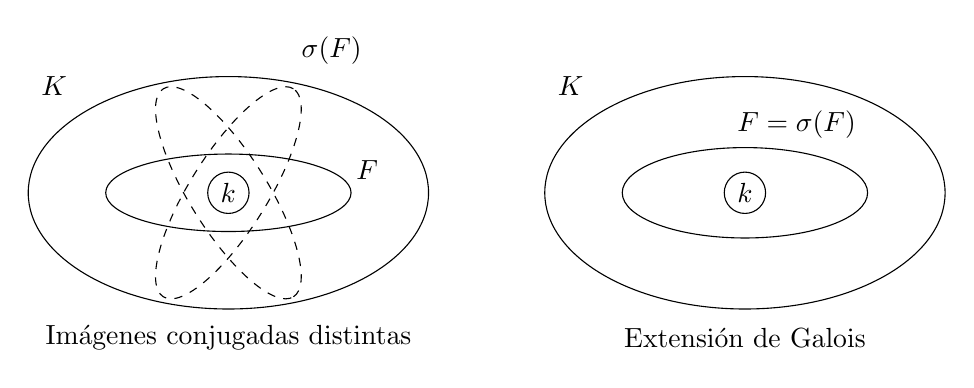
\begin{tikzpicture}[scale=.82]
\begin{scope}
\draw (0,0) ellipse (3.1 and 1.8);
\node at (-2.7,1.65) {$K$};
\draw (0,0) ellipse (1.9 and .6);
\draw[dashed,rotate=58] (0,0) ellipse (1.9 and .6);
\draw[dashed,rotate=-58] (0,0) ellipse (1.9 and .6);
\draw[fill=white] (0,0) circle (.32);
\node at (0,0) {$k$};
\node at (2.15,.35) {$F$};
\node at (1.6,2.2) {$\sigma(F)$};
\node at (0,-2.25) {Imágenes conjugadas distintas};
\end{scope}
\begin{scope}[xshift=8cm]
\draw (0,0) ellipse (3.1 and 1.8);
\node at (-2.7,1.65) {$K$};
\draw (0,0) ellipse (1.9 and .7);
\draw (0,0) circle (.32);
\node at (0,0) {$k$};
\node at (.8,1.05) {$F=\sigma(F)$};
\node at (0,-2.25) {Extensión de Galois};
\end{scope}
\end{tikzpicture}

\medskip
\begin{tikzpicture}[scale=.9]
\draw (0,0) ellipse (3.8 and 1.85);
\node at (-3.3,1.6) {$\mathbb C$};
\draw (.6,0) ellipse (2.05 and .65);
\draw[dashed,rojoDiagramaCIMAT,rotate=57] (0,0) ellipse (1.75 and .55);
\draw[dashed,rojoDiagramaCIMAT,rotate=-57] (0,0) ellipse (1.75 and .55);
\draw[fill=white] (0,0) circle (.34);
\node at (0,0) {$\mathbb Q$};
\node at (3.5,1.35) {$\mathbb Q(a)$};
\node[above=5pt] at (1.5,1.95) {$\mathbb Q(a\omega)$};
\node[below=5pt] at (1.5,-1.95) {$\mathbb Q(a\omega^2)$};
\end{tikzpicture}
